\section{Decay}

Radioactive decay is the change in the composition of a core by emitting particles and/or electro-magnetic radiation. Different kinds of radioactive decay are i.e. decay as a result of emission of negatrons or positrons and decay under emission of $\gamma$-rays.

\begin{tabbing}
\=xxxxxxxxxxxxxxxxxxxxxxx \=xxxxxxxxxxxxxxxxx \kill
\> $\alpha$-decay
\> ${^{232}_{\phantom{2}90}}\mathrm{Th}\rightarrow\;{^{228}_{\phantom{2}88}}\mathrm{Ra}+{^{4}_{2}}\mathrm{He}$ \\[1.5ex]
\> $\beta$-decay
\> ${^{228}_{\phantom{2}88}}\mathrm{Ra}\rightarrow\;{^{228}_{\phantom{2}89}}\mathrm{Ac}+{^{\phantom{-}0}_{-1}}\mathrm{e}$ \\[1.5ex]
\> $\gamma$-decay
\> ${^{236}_{\phantom{2}92}}\mathrm{U}^{\star}\rightarrow\;{^{236}_{\phantom{2}92}}\mathrm{U}+\gamma$
\end{tabbing}

The above given examples show that the radioactive decay is an irreversible process. The following differential equation describes the decay as first order reaction (without chain development):
\begin{equation}
\frac{\partial C}{\partial t}\,=\,-\lambda\cdot C
\label{eq55}
\end{equation}
{\small
with $\lambda$ - decay rate (s$^{-1}$).
}

The integration of this equation causes an exponential decay term in the following form.
\begin{equation}
C(t)\,=\,C_0\cdot e^{-\lambda\cdot t}
\label{eq56}
\end{equation}
{\small
with $C_0$ - initial concentration (kg$\cdot$m$^{-3}$).
}

The decay values are commonly expressed as the so-called half life ($t_{1/2}$). This is the point of time when half of the substance is degraded. The relation between the half-life $T$ and the decay rate results from:
\begin{equation}
e^{-\lambda\cdot t}\,=\,\frac{1}{2}\;\Rightarrow\;
\lambda\,=\,\frac{\ln(2)}{T}\,\cong\,\frac{0.693}{T}
\label{eq57}
\end{equation}

\subsection{Definition}

The aim of this example is to simulate the mass transport with the influence of decay, but without any sorption. At the left side of the considered aquifer there is a volume source of 0.1~m$^3$/d, at the right side there is a constant water pressure of 20 kPa. The tracer substance in the source volume is distributed by a stationary flow in the homogeneous aquifer. The mass distribution after 100 days has to be calculated. Figure \ref{fig51} shows a sketch of the calculation area.

\begin{figure}[htbp]
\centering
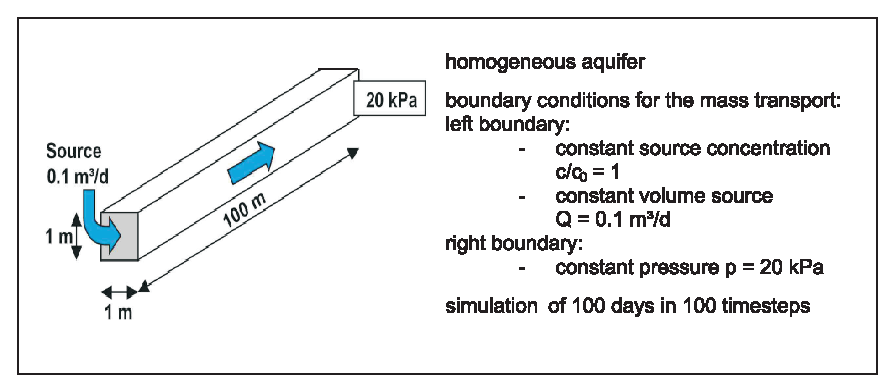
\includegraphics[width=1.0\textwidth]{PART_II/C/fig51.eps}
\caption{Calculation area: homogeneous aquifer}
\label{fig51}
\end{figure}

The following simplifications are assumed: (1) no sorption, exclusively decay of components (2) homogeneous aquifer, saturated, stationary flow.
%
For the 1-dimensional calculation the calculation area is simplified as a line of a length of 100~m with 100 elements and 101 nodes. As boundary conditions the relative concentration amounts 1 and the source volume of the fluid phase with 0.1~m$^3$/d is given at the left border of the calculation area and a constant pressure of 20 kPa at the right boundary. The used parameters of the soil are listed in Table \ref{tab51}. The calculation is divided into 100 time steps with a constant time step length of 1 day. That means, the flow and transport processes in the aquifer within 100 days are simulated.

\begin{table}[h]%[tab-ldhp]
\begin{center}
\begin{tabular}{llrr}
\toprule
Symbol & Parameter & Value & Unit \\
\midrule
$\Phi$ & Porosity & 0.2 & -- \\
$K$ & Permeability & 1.0$\cdot 10^{-12}$ & m$^2$ \\
$\rho$ & Density water & 1000 & kg/m$^{-3}$  \\		
$\eta$ & Viscosity water & 0.001 & Pa$\cdot$ s \\
$\alpha_L$ & Dispersion length & 5.0 & m \\
$\lambda$ & Decay in solved phase & 2.0$\cdot 10^{-7}$ & s$^{-2}$ \\
\bottomrule
\end{tabular}
\caption{Model parameters}
\label{tab51}
\end{center}
\end{table}

%\subsubsection*{Evaluation method}
The concentration distribution at a special point in time and over a given distance is calculated by equation (\ref{eq53}). Hereby the retardation coefficient is set equal to 1. The analytical solutions are depicted in Figure \ref{fig52} as single symbols.

\subsection{Results}

In Figure \ref{fig52} you can find the concentration distribution over the whole length of the 1~D model at the final simulation time of 100 days. Obviously, the numerical results meet well the analytical solutions.

\begin{figure}[htbp]
\centering
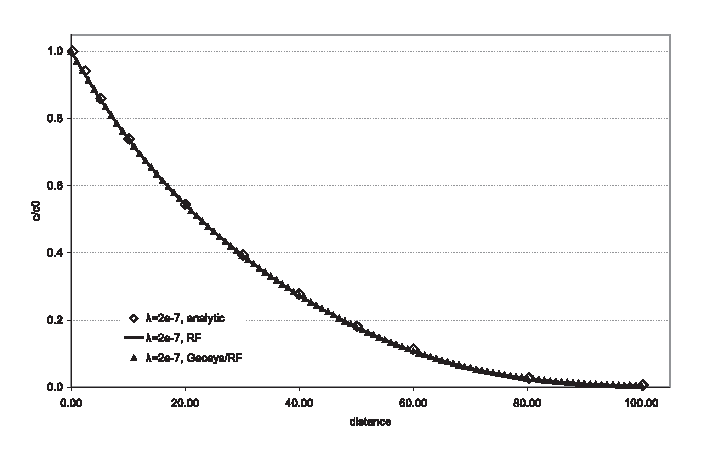
\includegraphics[width=0.8\textwidth]{PART_II/C/fig52.eps}
\caption{Concentration distribution after 100~d (decay)}
\label{fig52}
\end{figure}
